\documentclass[10pt, pscyr, nonums]{hedlabwork}
\usepackage[russian]{babel}
\usepackage[electricity]{hedphysics}
\usepackage{graphicx}
\graphicspath{{images/}, {plots/}}

\newgeometry{top=1.5cm, bottom=1.5cm, left=1cm, right=1cm}

\student{Слоква В. И., Ф-469}
\date{13.11.2013}
\labnum{601}
\labname{Определение электродвижущей силы термопары}

\begin{document}
  \makeheader

  \emph{Цель работы:} определение зависимости термоэлектродвижущей силы
  термопары от разности температур спаев.

  \emph{Используемые при расчетах формулы и значения:}
  \( \EMF_T = \alpha (T_2 - T_1) \), \( \Delta T = T_2 - T_1 \).

  \begin{figure}[h!]
    \center
    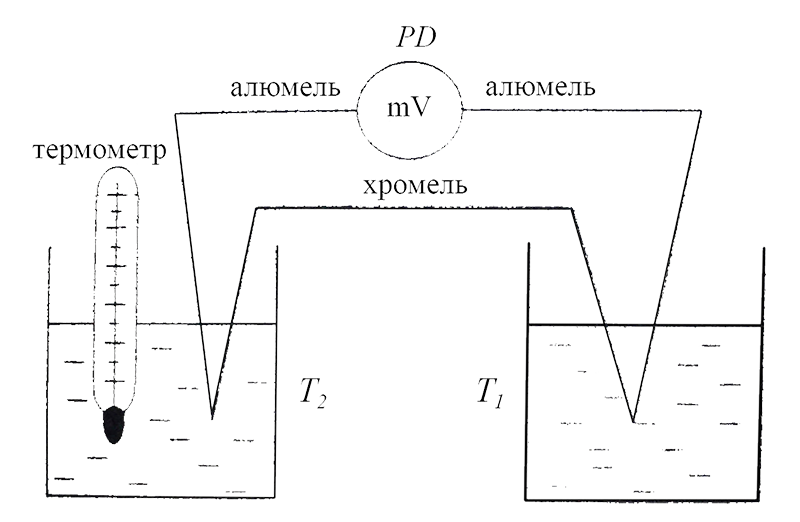
\includegraphics[width=.5\textwidth]{appearance} \\
    \parbox{.5\textwidth}{\caption{Внешний вид установки}}
  \end{figure}
  \vspace*{-2em}

  \begin{table}[h!]
    \center \caption{Результаты измерений}
    \begin{tabular}{|*{5}{C{.12}|}} \hline
      \( T_1 \), К & \( T_2 \), К & \( \Delta T \), К &
        \( \EMF_T \), В & \( \alpha \), В/К \\ \hline
      \multirow{9}{*}{295} &
        295 &  0 &   0 & \multirow{10}{*}{\( 71,\!4\cdot 10^{-6} \)} \\ \cline{2-4}
      & 303 &  8 & 0,5 & \\ \cline{2-4}
      & 313 & 18 & 1,2 & \\ \cline{2-4}
      & 323 & 28 & 2,0 & \\ \cline{2-4}
      & 333 & 38 & 2,7 & \\ \cline{2-4}
      & 343 & 48 & 3,4 & \\ \cline{2-4}
      & 353 & 58 & 4,2 & \\ \cline{2-4}
      & 363 & 68 & 4,8 & \\ \cline{2-4}
      & 369 & 74 & 5,2 & \\ \hline
    \end{tabular}
  \end{table}
\end{document}
